\documentclass[../sparc.tex]{subfiles}
\graphicspath{{\subfix{../images/}}}
\begin{document}

\section{Sound}
\index{Music!Sound frequency}
\newglossaryentry{Hz}{name=Hz, description={Hertz}}
\newglossaryentry{kHz}{name=kHz, description={Kilohertz ($10^3$ Hz)}}
\newglossaryentry{MHz}{name=MHz, description={Megahertz ($10^6$ Hz)}}
\newglossaryentry{GHz}{name=GHz, description={Gigahertz ($10^9$ Hz)}}

As it is commonly known, \emph{sound} is a mechanical disturbance from a state
of equilibrium that propagates through some medium (such as the air) in a form
of an acoustic wave. \cite{britannica:sound}

One of the main parameters of the sound is its \emph{frequency}.

Frequencies are measured in \emph{Hertz} (\gls{Hz}), and one Hertz (1 Hz) means
one oscillation per second.  10 oscillations per seconds gives us 10 Hz, 100
oscillations per second gives us 100 Hz and so on.  When we are talking about
1000 Hz or more, it is more convenient to use the standard multiples of a Hertz:
``Kilo-'' (\gls{kHz}), ``Mega-'' (\gls{MHz}) and ``Giga-'' (\gls{GHz}).

Some of the common multiples of a Hertz are shown in the table below.

\begin{table}[h]
  \centering
  \begin{tabular}{p{3cm}|p{4cm}|p{3.5cm}}
    Measurement unit & Relation to Hertz & Examples \\
    \hline \hline
    Hertz (Hz)
    & $ 1 \mbox{Hz} $ or $ 10^0 \mbox{Hz} $
    & $ 100 * 10^0 \mbox{Hz} = 100 \mbox{Hz} $ \\
    \hline
    Kilohertz (kHz)
    & $ 1000 \mbox{Hz} $ or $ 10^3 \mbox{Hz} $
    & $ 100 * 10^3 \mbox{Hz} = 100 \mbox{kHz} $ \\
    \hline
    Megahertz (MHz)
    & $ 1000000 \mbox{Hz} $ или $ 10^6 \mbox{Hz} $
    & $ 100 * 10^6 \mbox{Hz} = 100 \mbox{MHz} $ \\
    \hline
    Gigahertz (GHz)
    & $ 1000000000 \mbox{Hz} $ или $ 10^9 \mbox{Hz} $
    & $ 100 * 10^9 \mbox{Hz} = 100 \mbox{GHz} $ \\
  \end{tabular}
  \caption{Some units of the frequency measurement.}
  \label{table:sound-hertz-scale}
\end{table}

Thus we need to know the sound frequency to make an acoustic wave with proper
wave length to make that sound.  And vice versa, when we know the wave length,
we can calculate the sound frequency from it.  This can be visualized as is
shown on fig. \ref{fig:sound-fig-1}.

\begin{figure}[h]
  \centering
  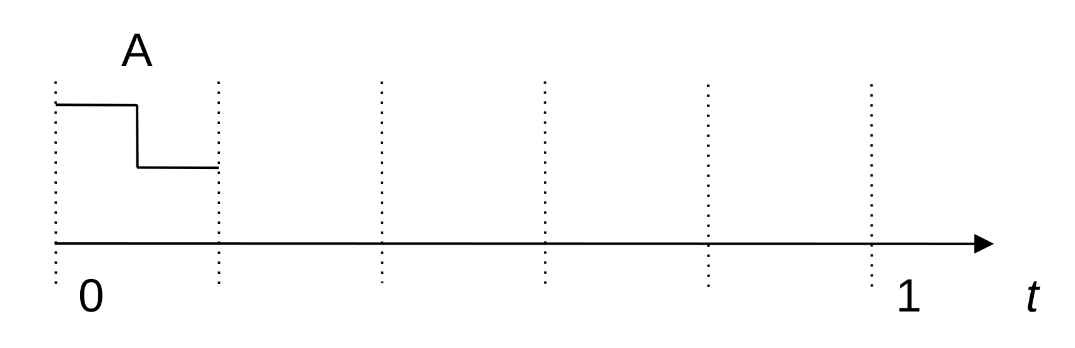
\includegraphics[width=10cm]{sound-fig-1}
  \caption{A visual representation of an acoustic wave with the frequency of 5
    Hz.}
  \label{fig:sound-fig-1}
\end{figure}

If we know that an oscillation can be fit 5 times in 1 second we say that the
frequency of such wave is 5 Hz.  If we want to calculate the period duration, we
can divide 1 second (specified in microseconds) by the frequency:

\begin{equation}
  \frac{1000000 \mu\mbox{s}}{5 \mbox{Hz}} = 200000 \mu\mbox{s}
\end{equation}

Which means that the wave length is 200000 $\mu\mbox{s}$, or $ 200 * 10^3
\mbox{ms}$.  If we know the wavelength and want to know the frequency we can
divide 1 second (in microseconds) by the wavelength and by that we will get the
frequency (in Hertz).  That's easy.

\figureSoundGraph{en}

The method of sound generation is similar to \gls{PWM}. The main difference is
that now we must change the wavelength, keeping the duty cycle constant, equal
to 0.5 (or 50\%.)  As the duty cycle is always constant, the duration of
\texttt{HIGH} and \texttt{LOW} signals is equal and we only need to calculate
the \texttt{d} delay.  The process of sound generation is visualized as a graph
on fig. \ref{fig:sound-graph}.

As with the case of PWM, we start from the writing a procedure that implements
the aforementioned principles.  We call this procedure \texttt{play\_tone} and
will allow us to generate a sound on a specified port with the specified
frequency and length.

Let's see what the procedure will accept as the parameters:
\begin{enumerate}
\item \texttt{port} -- the number of a digital port to which a speaker is
  connected.
\item \texttt{f} -- the frequency of the sound as the floating point value.
\item \texttt{t} -- the sound length in microseconds.
\end{enumerate}

In C++ language it should look like this:
\begin{minted}{cpp}
  void play_tone(int port, float f, long t) {
    // Procedure body.
  }
\end{minted}

The first step here is to calculate the wave oscillation period (in
microseconds) from by dividing a second (specified in microseconds) by the
specified frequency:

\begin{minted}{cpp}
  const long T = 1000000 / f;
\end{minted}

Next we will calculate the duration of the delay \texttt{d} -- for that we have
to divide the period \texttt{T} by 2 (or by multiplying it by 0.5) to get the
half-period:

\begin{minted}{cpp}
  long d = T / 2;
\end{minted}

Now we can calculate how many periods we have to repeat to create a sound of the
specified length \texttt{t}:

\begin{minted}{cpp}
  int count = t / T;
\end{minted}

We're almost done.  What's left is to write down a loop that will generate the
specified acoustic wave -- \texttt{for} loop comes very handy in this situation:

\begin{listing}[H]
  \begin{minted}{cpp}
    for (int i = 0; i < count; i++) {
      digitalWrite(port, HIGH);
      delayMicroseconds(d);
      digitalWrite(port, LOW);
      delayMicroseconds(d);
    }
  \end{minted}
  \label{listing:play-tone-cycle}
  \caption{The implementation of the loop for generating an acoustic wave with
    the specified parameters on a digital \texttt{port}.}
\end{listing}

The whole procedure is shown below:
\begin{listing}[H]
  \begin{minted}{cpp}
    void play_tone(int port, float f, long t) {
      const long T = 1000000 / f;
      long d = T / 2;
      int count = t / T;
      for (int i = 0; i < count; i++) {
        digitalWrite(port, HIGH);
        delayMicroseconds(d);
        digitalWrite(port, LOW);
        delayMicroseconds(d);
      }
    }
  \end{minted}
  \label{listing:play-tone-procedure}
  \caption{A simple procedure for generating a sound on an Arduino.}
\end{listing}

Our first version of the procedure for sound generation is finished.  Now we
have to connect a speaker to an Arduino and test it in action.

\note{In many cases one task can be solved in many ways.  For example, our
  \texttt{play\_tone} procedure can be implemented differently; our current
  version is just one of the correct ones.}

\end{document}
